\documentclass{article}
\usepackage{ifplatform}

\ifmacosx
\usepackage[fontset=mac]{ctex}
\fi
\iflinux
\usepackage[fontset=ubuntu]{ctex}
\fi

\usepackage{amsmath}
\usepackage{amssymb}
\usepackage{graphicx}
\usepackage{enumitem}
\usepackage{multicol}
\usepackage{multirow}

% http://kuing.orzweb.net/viewthread.php?tid=3004
\newcommand\rsx[1]{\left.{#1}\vphantom{\big|}\right|}

\title{Homework 4 - Malicious Comments Identification}
\author{資工系博士班二年級 D06922023 顏志軒}

\begin{document}

\maketitle

\textbf{Problem 1.} (0.5\%) 請說明你實作之 RNN 模型架構及使用的 word embedding 方法,回報模型的正確率並繪出訓練曲線 *。(0.5\%) 請實作 BOW+DNN 模型,敘述你的模型架構, 回報正確率並繪出訓練曲線。

\small* 訓練曲線 (Training curve): 顯示訓練過程的 loss 或 accuracy 變化。橫軸為 step 或 epoch,縱軸為 loss 或 accuracy。\normalsize

\textbf{Problem 2.} (1\%) 請敘述你如何 improve performance(preprocess, embedding, 架構等), 並解釋為何這些做法可以使模型進步。

\textbf{Problem 3.} (1\%) 請比較不做斷詞 (e.g., 以字為單位) 與有做斷詞,兩種方法實作出來的 效果差異,並解釋為何有此差別。

\textbf{Problem 4.} (1\%) 請比較 RNN 與 BOW 兩種不同 model 對於「在說別人白痴之前,先想想自己」與「在說別人之前先想想自己,白痴」這兩句話的分數 (model output),並討論造成差異的原因。

\textbf{Problem 5.} (1\%) In this exercise, we will train a binary classifier with AdaBoost algorithm on the data shown in the table. Please use decision stump as the base classifier. Perform AdaBoost algorithm for T = 3 iterations. For each iteration (t = 1, 2, 3), write down the weights $u_n^t$ used for training, the weighted error rate $\epsilon_t$, scaling coefficient $\alpha_t$, and the classification function $f_t(x)$. The initial weights $u_n^1$ are set to 1 (n = 0, 1, ..., 9). Please refer to the course slides for the definitions of the above notations. Finally, combine the three classifiers and write down the final classifier.

\begin{center}
\begin{tabular}{c|cccccccccc}
\hline
x & 0 & 1 & 2 & 3 & 4 & 5 & 6 & 7 & 8 & 9\\
y & + & - & + & + & + & - & - & + & - & -\\
\hline
\end{tabular}
\end{center}

\textbf{Problem 6.} (1\%) In this exercise, we will simulate the forward pass of a simple LSTM cell. Figure.1 shows a single LSTM cell, where $z$ is the cell input, $z_i, z_f, z_o$ are the control inputs of the gates, $c$ is the cell memory, and $f, g, h$ are activation functions. Given an input $x$, the cell input and the control inputs can be calculated by

\begin{equation*}
\begin{aligned}
  z &= w \cdot x + b\\
z_i &= w_i \cdot x + b_i\\
z_f &= w_f \cdot x + b_f\\
z_o &= w_o \cdot x + b_o
\end{aligned}
\end{equation*}

Where $w, w_i, w_f, w_o$ are weights and $b, b_i, b_f, b_o$ are biases. The final output can be calculated by

\begin{equation*}
y = f(z_o)h(c')
\end{equation*}

where the value stored in cell memory is updated by

\begin{equation*}
c' =f(z_i)g(z)+c f(z_f)
\end{equation*}

Given an input sequence $x_t (t = 1, 2, \ldots, 8)$, please derive the output sequence $y_t$. The input sequence, the weights, and the activation functions are provided below. The initial value in cell memory is 0. Please note that your calculation process is required to receive full credit.

\begin{multicols}{2}
\begin{equation*}
\begin{aligned}
w   &= [0, 0, 0, 1] &, b = 0\\
w_i &= [100, 100, 0, 0] &, b_i = -10\\
w_f &= [-100, -100, 0, 0] &, b_f = 110\\
w_o &= [0, 0, 100, 0] &, b_o = -10 
\end{aligned}
\end{equation*}

\begin{tabular}{c|cccccccc}
t & 1 & 2 & 3 & 4 & 5 & 6 & 7 & 8\\
\hline
\multirow{4}{*}{$x_t$} & 0 & 1 & 1 & 0 & 0 & 0 & 1 & 1\\
& 1 & 0 & 1 & 1 & 1 & 0 & 1 & 0\\
& 0 & 1 & 1 & 1 & 0 & 1 & 1 & 1\\
& 3 & -2 & 4 & 0 & 2 & -4 & 1 & 2
\end{tabular}

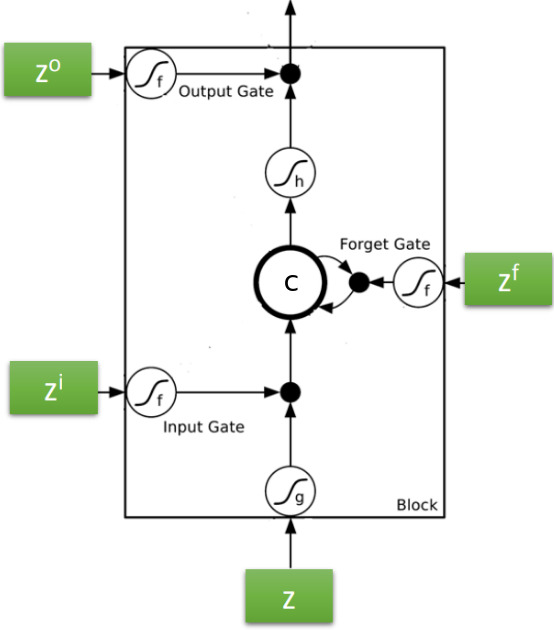
\includegraphics[width=0.4\textwidth]{image-002.jpg}

\end{multicols}

\end{document}
